\chapter*{Нерешённые головоломки}

\setlength{\epigraphwidth}{.55\textwidth}
\epigraph{Человек не может учиться иначе, как двигаясь от известного к неизвестному.}{---Клод Бернар (1813---1878)}

Цитируя моего приятеля: «Нерешённая головоломка --- это что ещё за хрень такая?».
Действительно, невозможно узнать, имеет ли задача изящное решение, пока она не решена.
Тем не менее, некоторые нерешённые задачи привлекают красотой и простотой своей постановки, удивляя при этом тем, что решение неизвестно.
Математики, особенно такие, как и ваш автор, воспитанные в эрдёшовской традиции искать самое простое из непонятного, часто бравируют такими головоломками.
Соберите несколько таких фанатиков вместе, и вы услышите разговор вроде такого:

«Вот что меня беспокоит; ты знаешь ответ?»

«На самом деле, я даже не уверен, что знаю ответ на этот более простой вопрос.»

«Вы шутите? \emph{Я} даже не знаю \emph{вот этого}!»

Конечно, следует различать нерешённую головоломку и гипотезу, как, например, гипотезу Римана или P=NP.
Гипотезы могут не иметь красивой и элементарной формулировки, но они возникают на пути к истине (часто как препятствия) и поэтому их изучают.
Формулировка гипотезы часто требует «профессиональных» математических понятий (графы, группы, многообразия, преобразования, представления и тому подобное), которые не допускаются в головоломке, хотя они могут подразумеваться или быть необходимыми в её решении.

Нерешённые головоломки могут быть развлекательными, интригующими и даже пакостными,
но они не должны быть принципиально важны, \emph{по крайней мере, это не должно быть известно}.
Конечно, каждая нерешённая задача важна как пробел в нашем знании.
Её решение может натолкнуть на создание полезной техники;
или она может решиться приложением глубокой математики.
При этом некоторые задачи, приведённые ниже, такие, как гипотеза Франкла или $3x+1$ дилемма, привлекли столько внимания, что любое решение будет представлять значительный интерес, независимо от применимости его в других областях.

Эти задачи представлены здесь для развлечения и чтобы напомнить вам о том, как мало мы знаем.
Если даже одну из них кто-то решит, узнав про неё в этой книге, то случится небольшое чудо.
Если вам кажется, что вы решили одну из них, то скорее всего, вы ошибаетесь.
Воспользуйтесь приведенными ссылками, вашими профессиональными математическими друзьями и вашей любимой поисковой системой в интернете, чтобы узнать больше о других попытках решить эту задачу.
Скорее всего вы узнаете, что попали в известную ловушку, и не опозоритесь на публике.

Если же вы все еще считаете, что у вас есть настоящее решение, то оно должно быть записано и отправлено в подходящий математический журнал.
Не отправляйте его мне: я не эксперт ни в одной из задач.

\medskip

В этой главе, конечно, не будет раздела решений, но мы продолжим формат: формулировки сначала, а комментарии и ссылки потом.
Начнем с классики от Джона Конвея.
Удачи!


\subsection*{Ангел и Дьявол Конвея}

Ангел летает над бесконечной шахматной доской, и время от времени должен садиться на клетку.
Он может пролететь не более 1000 ходов короля до очередного приземления.

Пока Ангел летит, Дьявол, живущий под доской, может уничтожить одну клетку по своему выбору.

Может ли Дьявол поймать Ангела?

\subsection*{$\bm{3x+1}$ дилемма}

Начиная с произвольного положительного целого числа, будем повторять следующее действие: если оно чётно, то сократим его вдвое, а если нечётно, утроим его и добавим 1.

Доказать, что в конце концов мы зациклимся; или даже сильнее, что в конечном итоге придём к циклу $1, 4, 2, 1, 4, 2,\dots$.

\subsection*{Самая длинная общая подпоследовательность}
Генерируются две случайные двоичные последовательности длиной $n$, причём каждая цифра определяется независимо и равна 1 с вероятностью $p$.
Пусть $C_p(n)$ есть средняя длина самой длинной общей подпоследовательности в обоих, и пусть $C_p$ есть предел отношения $C_p(n)/n$.

Вычислите $C_{\frac12}$ или, по крайней мере, докажите, что $C_{\frac12}<C_{p}$ при $p\ne\tfrac12$.

\subsection*{Квадратура озера}

Докажите, что каждая простая замкнутая кривая на плоскости содержит четвёрку точек в вершинах квадрата.

\subsection*{Одинокий бегун}

Бегуны  стартуют в одной точке и бегут по круговой дорожке единичной длины;
каждый бежит с постоянной скоростью и скорости у всех различны.

Доказать, что каждый бегун в какой-то момент времени будет на расстоянии хотя бы $1/n$ от любого другого бегуна.

\subsection*{Сортировка шаров}

В ряд стоит $n$ корзинок с парой шаров в каждой, при чём в $i$-той корзинке лежат шары с номерами $n+1-i$.
За одну операцию разрешается поменять два шара в соседних корзинках.

Сколько операций необходимо для того, чтобы каждый шар попал в корзинку со своим номером?

\begin{figure}[h!]
\centering
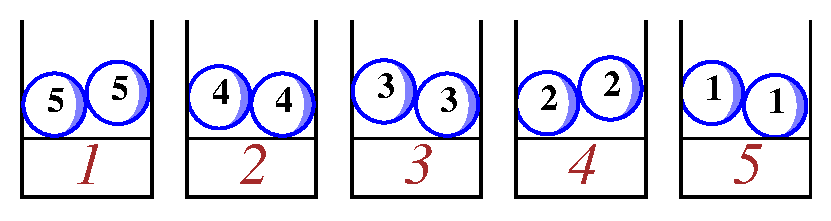
\includegraphics[scale=0.5]{Figs/UnsolvedPuzzles/bins}
\end{figure}

\subsection*{Развёртка многогранника}

Доказать, что произвольный выпуклый многогранник можно разрезать по рёбрам, так что полученную поверхность можно развернуть в плоский многоугольник.

\subsection*{Освещение многоугольника}

Любой ли многоугольник с зеркальными сторонами можно осветить одной лампочкой горящей в некоторой его внутренней точке?

\subsection*{Треклы Конвея}

Треклом называют диаграмму на плоскости, состоящей из вершин и рёбер (кривых без самопересечений), такую что:
\begin{itemize}
\item каждое ребро начинается и заканчивается в двух различных вершинах, и не проходит через другие вершины; и
\item любая пара рёбер пересекает друг друга ровно один раз, либо в общей вершине, либо во внутренней точке.
\end{itemize}

Существует ли трекл с б\'{о}льшим числом рёбер, чем вершин?

\begin{figure}[h!]
\centering
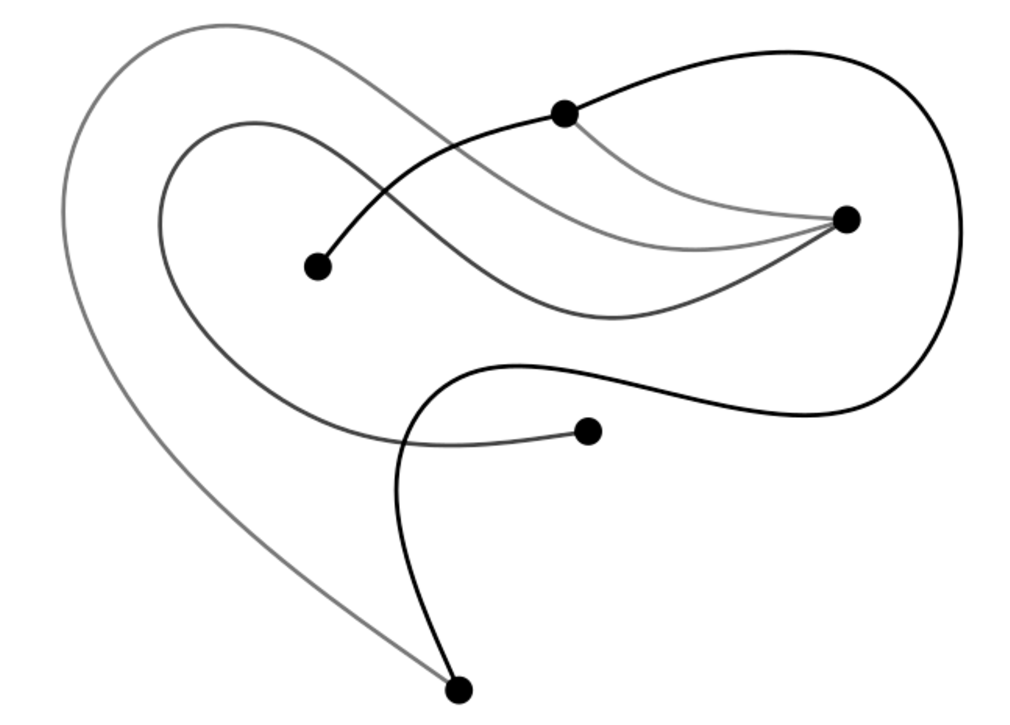
\includegraphics[scale=0.5]{Figs/UnsolvedPuzzles/thrack}
\end{figure}

\subsection*{Затор}

Вершины бесконечной решётки на плоскости выбираются независимо с фиксированной вероятностью $p\in (0,1)$.
В каждую из выбранных вершин помещают автомобиль направленный либо на север либо на восток,
в каждом  случае направление выбирается независимо подкидыванием монетки.

Движение регулируется светофорами, которые включают поочерёдно «зеленый-восточный» и «зеленый-северный».
При включённом зеленом-восточном, каждый восточный автомобиль, правая соседняя вершина от которого не занята, перемещается в эту вершину; остальные (в том числе заблокированные другим восточным автомобилем) остаются там, где они находились.

Когда включается зеленый-северный, каждый незаблокированный автомобиль в северном направлении перемещается на одну вершину в северном направлении.

Эксперименты говорят, что если $p$ ниже определённого критического значения $p_0$,
то автомобили постепенно разъезжаются.
Более того каждый автомобиль имеет предельную среднюю скорость, равную скорости автомобиля, который никогда не блокируется.
Но когда $p> p_0$ происходит обратное: автомобили попадают в безнадёжный затор, то есть каждый автомобиль делает только конечное число переездов, и останавливается навсегда.

Если вы готовы в это поверить, попробуйте доказать одно из этих утверждений.

\subsection*{Средние уровни}

Докажите, что все подмножества размера $n$ или $n+1$ в множестве размера $2n+1$, можно обойти циклически добавляя или удаляя по одному элементу за раз.

\subsection*{Построение диаграмм Венна}

Диаграмма Венна порядка $n$ представляет собой набор из $n$ простых замкнутых кривых на плоскости, с трансверсальнымии пересечениями  по две кривых в точке и %???
таких, что для любого поднабора кривых множество точек внутри кривых из поднабора, и снаружи остальных кривых является непустым и связным.

Любую ли диаграмму Венна порядка $n$ можно ли расширить до диаграммы Венна порядка $n+1$?

\subsection*{Стратегия для игры в щёлк}

Алиса и Боб играют в следующую игру:
Фиксируется число $k$.
Алиса называет делитель $k$.
Боб называет другой делитель $k$, который не кратен последнему числу названным Алисой.
Алиса называет третий делитель, который не является кратным ни одному из уже назаванных; 
и так далее.
Проигравает тот, кто называет 1.

Обратите внимание, что при $k=2^{n}3^{m}$, эта игра эквивалентна игре щёлк из предыдущей главы для плитки шоколада $(m+1)\z\times (n+1)$.
То же рассуждение показывает, что у Алисы существует выигрышная стратегия, но остаётся следующая задача, как для версии с шоколадкой, так и для приведённого обобщения:

Найдите выигрышную стратегию для Алисы!

\subsection*{Все дороги ведут в Рим}

Дана сеть (не обязательно плоская) из городов и односторонних дорог со следующими свойствами:
из каждого города выходят ровно две дороги, и для некоторого фиксированного $n$, можно добраться из любого города в любой другой город пройдя по $n$ дорогам.

Докажите, что можно раскрасить дороги в красный и синий цвет таким образом, что (а) каждый город имеет выездную дорогу каждого цвета, и (б) есть набор инструкций (например, КССКК), который всегда заканчивается в одном и том же городе, независимо от исходного города.

\subsection*{Круги в круге}

Докажите, что любой набор кругов с общей площадью $1$ можно упаковать в круг площади $2$.
Ещё лучше доказать, что в $d$-мерном пространстве любой набор из подобных копий выпуклого тела, с общим объёмом 1, можно упаковать в подобную копию объёма $2^{d-1}$.

\subsection*{Гипотеза Франкла}

Пусть $U$ --- конечное множество, а $T$ --- семейство непустых подмножеств в $U$, замкнутое относительно объединения.
Докажите, что в $U$ есть элемент, принадлежащий, по меньшей мере, половине множеств в $T$.
